\section{Raspuns automat}

Mi-am comandat pizza si ajunge in timp ce folosesc pistolul de lipit. Prin urmare voi programa interfonul sa raspunda si sa deschida automat usa la urmatorul apel.

\begin{figure}[H]
\begin{center}
  \subfloat[Apasarea butonului albastru auto-answer va arata meniul pentru configurarea functionalitatii]{\label{fig:autoanswera}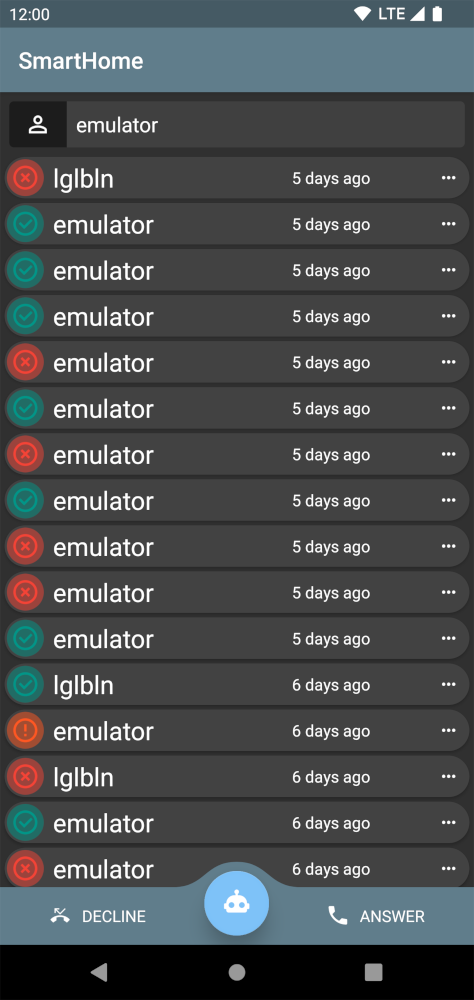
\includegraphics[width=\doublefigure]{05/01_android_autoanswer.png}}
  \hfil
  \subfloat[Alegerea unui interval pentru care functia va fi activa]{\label{fig:autoanswerb}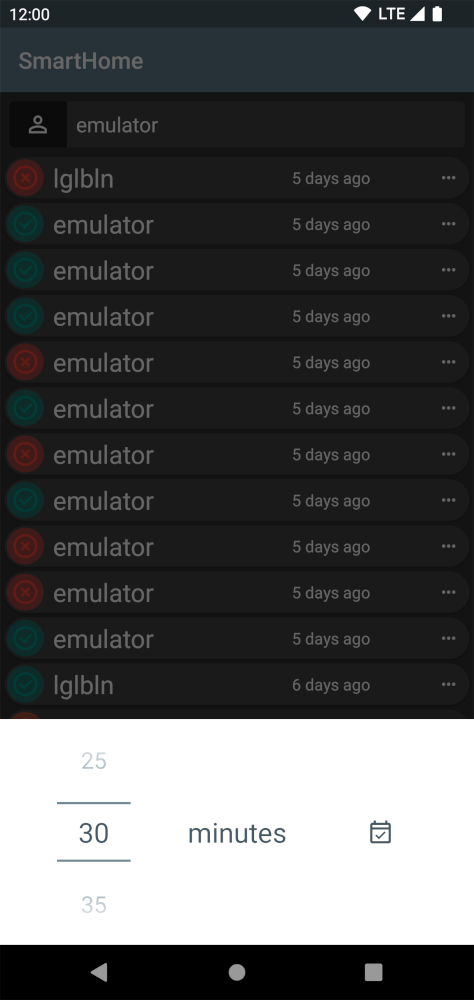
\includegraphics[width=\doublefigure]{05/02_android_auto_set.png}}
  \caption{Pasi pentru setare functie auto-answer}
  \label{fig:autoanswer}
\end{center}
\end{figure}

Se confirma ca functia este activata prin colorarea butonului auto-answer in portocaliu. Intr-o maniera similiara, daca se doreste oprirea inainte de termen, se poate face acest lucru din meniul anterior.

\section{Raspuns de la distanta}

Mi-am pierdut cartela standard \acrfull{rfid} pentru a intra in bloc. Asadar, voi suna la numerul apartamentului meu si voi folosi aplicatia mobila pentru a raspunde la propriul apel.